\documentclass{beamer}
\usetheme{CambridgeUS}
\usepackage[absolute,overlay]{textpos}
\usepackage{graphicx}
\usepackage{tikz}
\usepackage{animate}
\usepackage{calc}
\newcounter{m} % Number of sides of the polygon
\setcounter{m}{2}
\newcounter{c} % Internal Control Counter
\usepackage{hyperref}
\hypersetup{pdfpagemode=FullScreen}
\usefonttheme{professionalfonts}
\usepackage{smartdiagram}
\usepackage{times}
\usepackage{changepage}
\providecommand\thispdfpagelabel[1]{}

\usepackage{amssymb}
\usetikzlibrary{arrows.meta}
\usepackage{tikz}
\usepackage{amsmath}
\usepackage{verbatim}
\usetikzlibrary{arrows,shapes}
\usepackage{array,multirow,makecell}
\setcellgapes{1pt}
\makegapedcells
\newcolumntype{R}[1]{>{\raggedleft\arraybackslash }b{#1}}
\newcolumntype{L}[1]{>{\raggedright\arraybackslash }b{#1}}
\newcolumntype{C}[1]{>{\centering\arraybackslash }b{#1}}
\tikzset{
pil/.style={
           ->,
           thick,
           shorten <=2pt,
           shorten >=2pt,}}
\usetikzlibrary{arrows,shapes}
\usetikzlibrary{arrows,positioning}
\usepackage{smartdiagram}
\usepackage{metalogo}
\setbeamertemplate{headline}{}
\tikzstyle{vecArrow} = [thick, decoration={markings,mark=at position
   1 with {\arrow[semithick]{open triangle 60}}},
   double distance=1.4pt, shorten >= 5.5pt,
   preaction = {decorate},
   postaction = {draw,line width=1.4pt, white,shorten >= 4.5pt}]
\tikzstyle{innerWhite} = [semithick, white,line width=1.4pt, shorten >= 4.5pt]

\setbeamertemplate{navigation symbols}{}
\makeatletter
\setbeamertemplate{footline}
{
  \leavevmode%
  \hbox{%
  \begin{beamercolorbox}[wd=.333333\paperwidth,ht=2.25ex,dp=1ex,center]{author in head/foot}%
    \usebeamerfont{author in head/foot} {Onur, Bastien, Paul, Florent}
  \end{beamercolorbox}%
  \begin{beamercolorbox}[wd=.333333\paperwidth,ht=2.25ex,dp=1ex,center]{title in head/foot}%
    \usebeamerfont{title in head/foot}\insertsection
  \end{beamercolorbox}%
  \begin{beamercolorbox}[wd=.333333\paperwidth,ht=2.25ex,dp=1ex,right]{date in head/foot}%
    \usebeamerfont{date in head/foot}\insertshortdate{}\hspace*{2em}
    \insertframenumber{} / \inserttotalframenumber\hspace*{2ex} 
  \end{beamercolorbox}}%
  \vskip0pt%
}
\makeatother

\newcommand{\margin}{0\paperwidth}


%\beamersetrightmargin{\margin}
%\beamersetleftmargin{\margin}

\newcommand\Wider[2][3em]{%
\makebox[\linewidth][c]{%
  \begin{minipage}{\dimexpr\textwidth+#1\relax}
  \raggedright#2
  \end{minipage}%
  }%
}



\usetikzlibrary{shapes,snakes}

%\input{tex_files/ZZ_newcommand1}

\definecolor{myblue}{RGB}{79,129,189}

\tikzset{%
  >={Latex[width=2mm,length=2mm]},
  % Specifications for style of nodes:
            base/.style = {rectangle, rounded corners, draw=black,
                           minimum width=4cm, minimum height=1cm,
                           text centered, font=\normalfont},
  activityStarts/.style = {base, fill=blue!30},
       startstop/.style = {base, fill=red!30},
    activityRuns/.style = {base, fill=green!30},
         process/.style = {base, minimum width=2.5cm, fill=orange!15,
                           font=\normalfont},
}



\begin{document}

%\usepackage{framed}
%\usepackage{cite,url}
%\usepackage{amsmath,amssymb}
%\usepackage{amscd}
%\usepackage[english] {babel}
%\usepackage[pdftex]{graphicx,color}
%\usepackage{stmaryrd}
%\usepackage{amsmath}
%\usepackage{xspace,calc}
%\usepackage{games}
%\usepackage{booktabs}
%\usepackage{needspace}
%\use package{times}
%\usepackage{algorithmicx} % sorry

\bibliography{abbrev3,crypto,add,add2}


\title{Using NetZob for Active protocol reverse engineering }   
\author{Onur Catakoglu , Bastien Drouot, Paul Germouty, Florent Tardif} 
\date{November 2, 2017} 


\logo{%
    
\includegraphics[width=2cm,height=1cm,keepaspectratio]{zoby.png}%
    
\includegraphics[width=2cm,height=1cm,keepaspectratio]{redocsFullColor-W.png}~%
   
}

%\logo{\includegraphics[height=5mm]{limoges.jpg}}

\begin{frame}

	\titlepage
\end{frame}


%%%%%%%%%%%%%%%%%%%%%%%%%%%%%%%%%%%%%%%%%%



\begin{frame}


	\tableofcontents

\end{frame}

\section{Introduction}
\begin{frame}

	\tableofcontents[currentsection]
\end{frame}

\begin{frame}{Objectives-Attack Model}
\begin{itemize}
\item Reverse engineering transmission protocols

$\Rightarrow$ characterize protocols' structure

\item Client-owning Model

$\Rightarrow$ possibility to discuss with the server with the protocol
\end{itemize}
\end{frame}

\begin{frame}{Previous Work \textbf{Netzob}}
Passive framework for analysing transmission
\begin{itemize}
\item symbol
\item \textit{Format.splitStatic(s)}: align static set of field at the same position
\item \textit{Format.splitAligned(s)}: align static set of bytes 
\item \textit{Format.splitDelimiter(s,Raw($listofbytes$))}: separate fields with the given delimiters
\item \textit{Channel.Write}: allow sending TCP message to the server
\end{itemize}


\end{frame}

\begin{frame}{Exemples}
symbol screen shot
\end{frame}

\begin{frame}{Exemples}
Aligned screen shot
\end{frame}

\begin{frame}{Exemples}
Static screen shot
\end{frame}

\begin{frame}{Exemples}
Delimiter screen shot
\end{frame}

\section{RoadMap}
\begin{frame}

	\tableofcontents[currentsection]
\end{frame}

\begin{frame}{Road Map of GoodGuy ReverseIngBoy}
%%\begin{enumerate}
%%\item Sorting Input
%%
%%\bigskip
%%
%%\item Delimiting fields
%%
%%\bigskip 
%%
%%\item Characterizing fields
%%
%%\bigskip
%%
%%\item Assessing impact of the fields
%%
%%\bigskip
%%
%%\item Verifying hypothesis made in 3 and 4
%%\end{enumerate}
%\begin{center}
%\scalebox{0.7}{
%\smartdiagram[priority descriptive diagram]{
%  Verifying hypothesis made in 3 and 4,
%  Assessing impact of the fields,
%  Characterizing fields,
%  Delimiting fields,
%  Sorting Input}}
%\end{center}

%\begin{frame}
\begin{center}
\scalebox{0.9}{
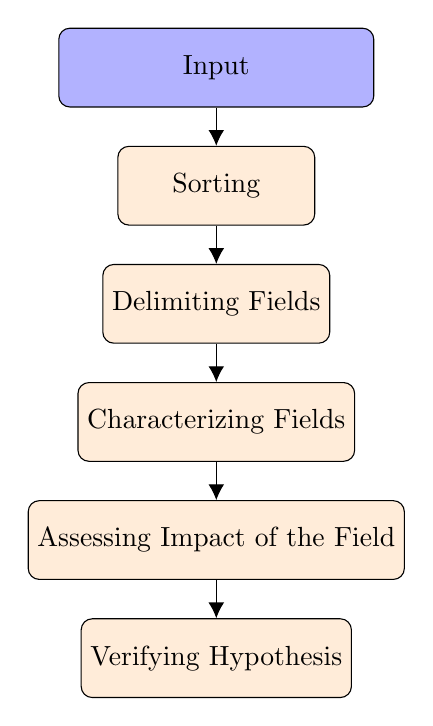
\begin{tikzpicture}[node distance=1.5cm,
    every node/.style={fill=white, font=\sffamily}, align=center]

\node (Input)             [activityStarts]              {Input};

\node (SI)     [process, below of=Input]          {Sorting};

\node (DF)     [process, below of=SI]          {Delimiting Fields};

\node (CF)     [process, below of=DF]          {Characterizing Fields};

\node (AI)     [process, below of=CF]          {Assessing Impact of the Field};

\node (VH)     [process, below of=AI]          {Verifying Hypothesis};

\draw[->]             (Input) -- (SI);
\draw[->]             (SI) -- (DF);
\draw[->]             (DF) -- (CF);
\draw[->]             (CF) -- (AI);
\draw[->]             (AI) -- (VH);
  \end{tikzpicture}}
  \end{center}



\end{frame}



\begin{frame}{Sorting Input}
\begin{center}
\scalebox{0.9}{
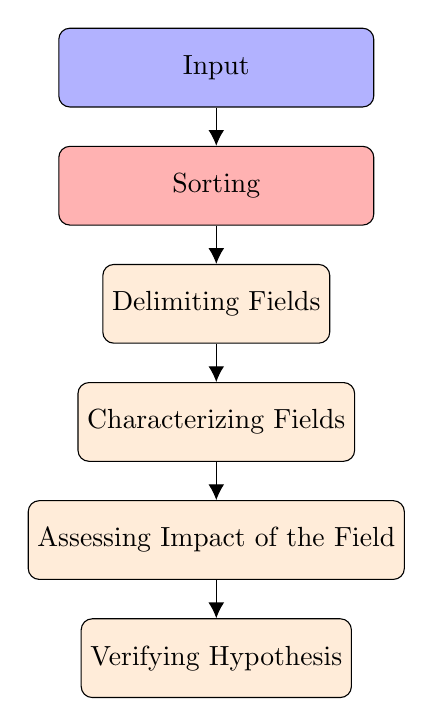
\begin{tikzpicture}[node distance=1.5cm,
    every node/.style={fill=white, font=\sffamily}, align=center]

\node (Input)             [activityStarts]              {Input};

\node (SI)     [startstop, below of=Input]          {Sorting};

\node (DF)     [process, below of=SI]          {Delimiting Fields};

\node (CF)     [process, below of=DF]          {Characterizing Fields};

\node (AI)     [process, below of=CF]          {Assessing Impact of the Field};

\node (VH)     [process, below of=AI]          {Verifying Hypothesis};

\draw[->]             (Input) -- (SI);
\draw[->]             (SI) -- (DF);
\draw[->]             (DF) -- (CF);
\draw[->]             (CF) -- (AI);
\draw[->]             (AI) -- (VH);
  \end{tikzpicture}}
  \end{center}
\end{frame}



\begin{frame}{Divide and Conquer}
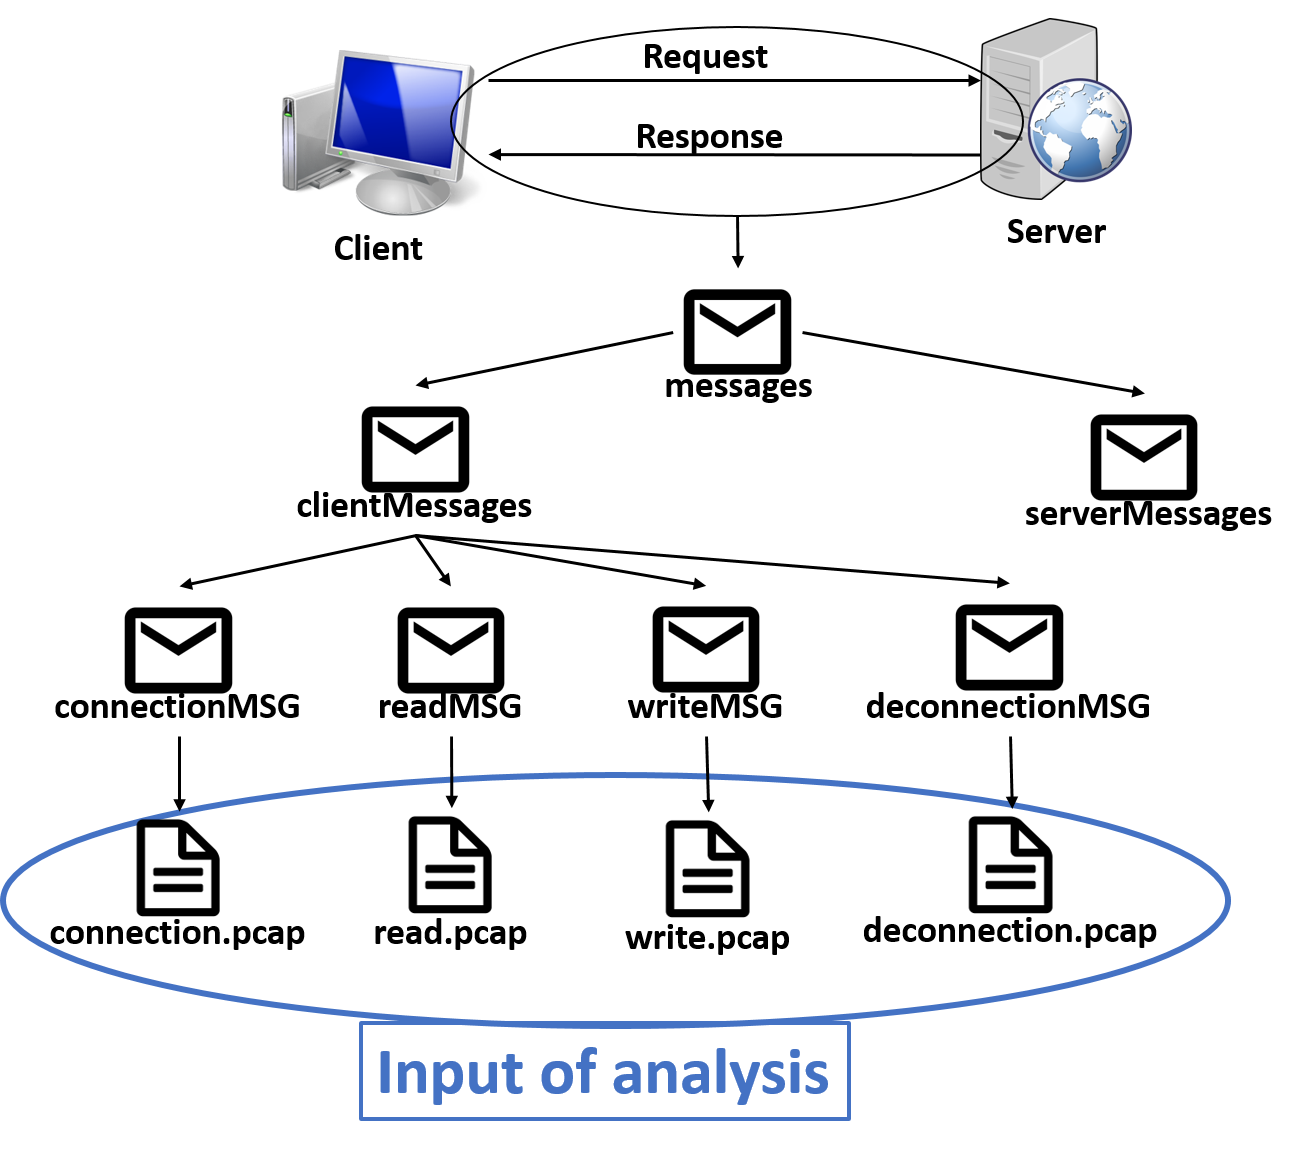
\includegraphics[scale=0.25]{Sorting_by_type.png}

\end{frame}


%\section{Basic Tools}
%\begin{frame}
%
%	\tableofcontents[currentsection]
%\end{frame}
%
%\begin{frame}
%getting pcap
%
%sorting pcap
%
%verify cruciality
%
%verify timeout
%
%send 1 message
%...
%
%
%\end{frame}
\begin{frame}{Delimiting Fields}
\begin{center}
\scalebox{0.9}{
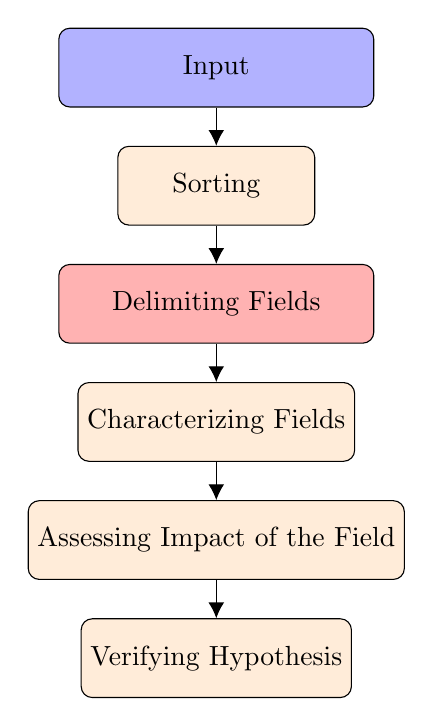
\begin{tikzpicture}[node distance=1.5cm,
    every node/.style={fill=white, font=\sffamily}, align=center]

\node (Input)             [activityStarts]              {Input};

\node (SI)     [process, below of=Input]          {Sorting};

\node (DF)     [startstop, below of=SI]          {Delimiting Fields};

\node (CF)     [process, below of=DF]          {Characterizing Fields};

\node (AI)     [process, below of=CF]          {Assessing Impact of the Field};

\node (VH)     [process, below of=AI]          {Verifying Hypothesis};

\draw[->]             (Input) -- (SI);
\draw[->]             (SI) -- (DF);
\draw[->]             (DF) -- (CF);
\draw[->]             (CF) -- (AI);
\draw[->]             (AI) -- (VH);
  \end{tikzpicture}}
  \end{center}
\end{frame}

%
\begin{frame}{Delimiters}
\begin{itemize}
\item Statistical research

\bigskip

\item Active verification

\bigskip

\item Double elimination
\end{itemize}

\end{frame}

\begin{frame}{Delimiters using}
screenshots
\end{frame}

\begin{frame}{SmartAligned}
ALLO BASTIEN
\end{frame}

\begin{frame}{SmartAligned}
screenshot
\end{frame}



\begin{frame}{Characterizing Fields}
\begin{center}
\scalebox{0.9}{
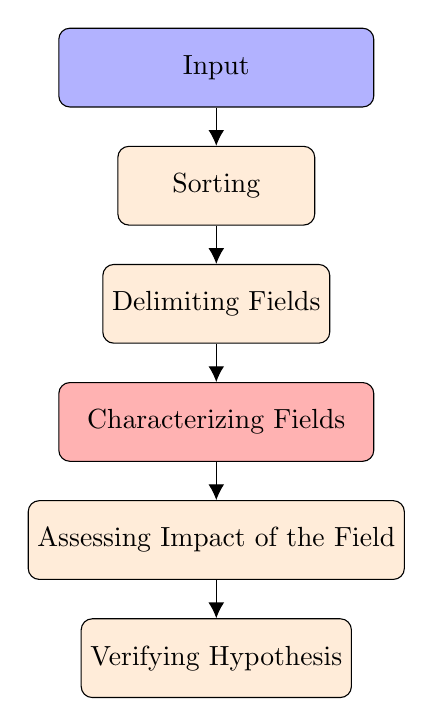
\begin{tikzpicture}[node distance=1.5cm,
    every node/.style={fill=white, font=\sffamily}, align=center]

\node (Input)             [activityStarts]              {Input};

\node (SI)     [process, below of=Input]          {Sorting};

\node (DF)     [process, below of=SI]          {Delimiting Fields};

\node (CF)     [startstop, below of=DF]          {Characterizing Fields};

\node (AI)     [process, below of=CF]          {Assessing Impact of the Field};

\node (VH)     [process, below of=AI]          {Verifying Hypothesis};

\draw[->]             (Input) -- (SI);
\draw[->]             (SI) -- (DF);
\draw[->]             (DF) -- (CF);
\draw[->]             (CF) -- (AI);
\draw[->]             (AI) -- (VH);
  \end{tikzpicture}}
  \end{center}
\end{frame}

\begin{frame}{Characterizing Fields}
\begin{itemize}
\item Static / Dynamic

\bigskip

\item Txt / Bin
\end{itemize}
\end{frame}



\begin{frame}{Assessing the Impact of the Fields}
\begin{center}
\scalebox{0.9}{
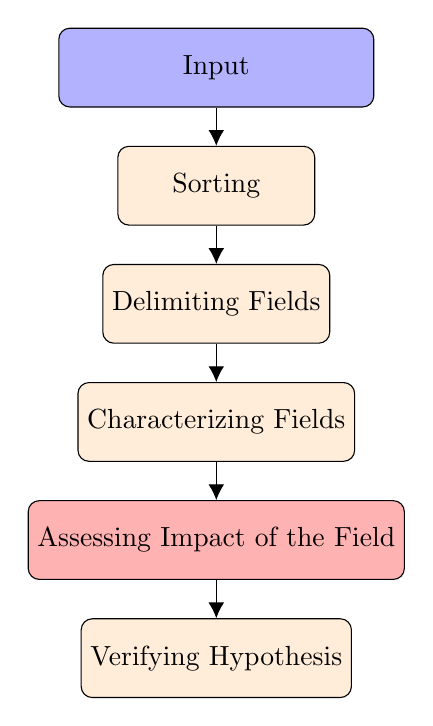
\begin{tikzpicture}[node distance=1.5cm,
    every node/.style={fill=white, font=\sffamily}, align=center]

\node (Input)             [activityStarts]              {Input};

\node (SI)     [process, below of=Input]          {Sorting};

\node (DF)     [process, below of=SI]          {Delimiting Fields};

\node (CF)     [process, below of=DF]          {Characterizing Fields};

\node (AI)     [startstop, below of=CF]          {Assessing Impact of the Field};

\node (VH)     [process, below of=AI]          {Verifying Hypothesis};

\draw[->]             (Input) -- (SI);
\draw[->]             (SI) -- (DF);
\draw[->]             (DF) -- (CF);
\draw[->]             (CF) -- (AI);
\draw[->]             (AI) -- (VH);
  \end{tikzpicture}}
  \end{center}
\end{frame}

\begin{frame}{Fields Order Importance}

\end{frame}

\begin{frame}{Finding Incrementation }
\end{frame}





\begin{frame}\frametitle{Stateless vs. Stateful}

  Stateful: messages depends on a global state $\Rightarrow$ need to understand the session mechanism beforehand

  ~

  Stateless: we can perform analysis on each message taken separately

  ~

  \begin{block}{Detection}
    \begin{itemize}
      \item get a valid message
      \item replay the message several time
      \item same messages ? \begin{tabular}{ccc}YES &$\Rightarrow$& stateless\\NO &$\Rightarrow$& stateful\end{tabular}
    \end{itemize}
  \end{block}
\end{frame}

\begin{frame}{Fuzzing}

  Impact of modifications in the messages

  \begin{itemize}
    \item identify the type of the fields (static or dynamic)
    \item take a message with a dynamic field
    \item query the server with both the original and modified message
    \item calculate the difference between the two
  \end{itemize}

  \begin{center}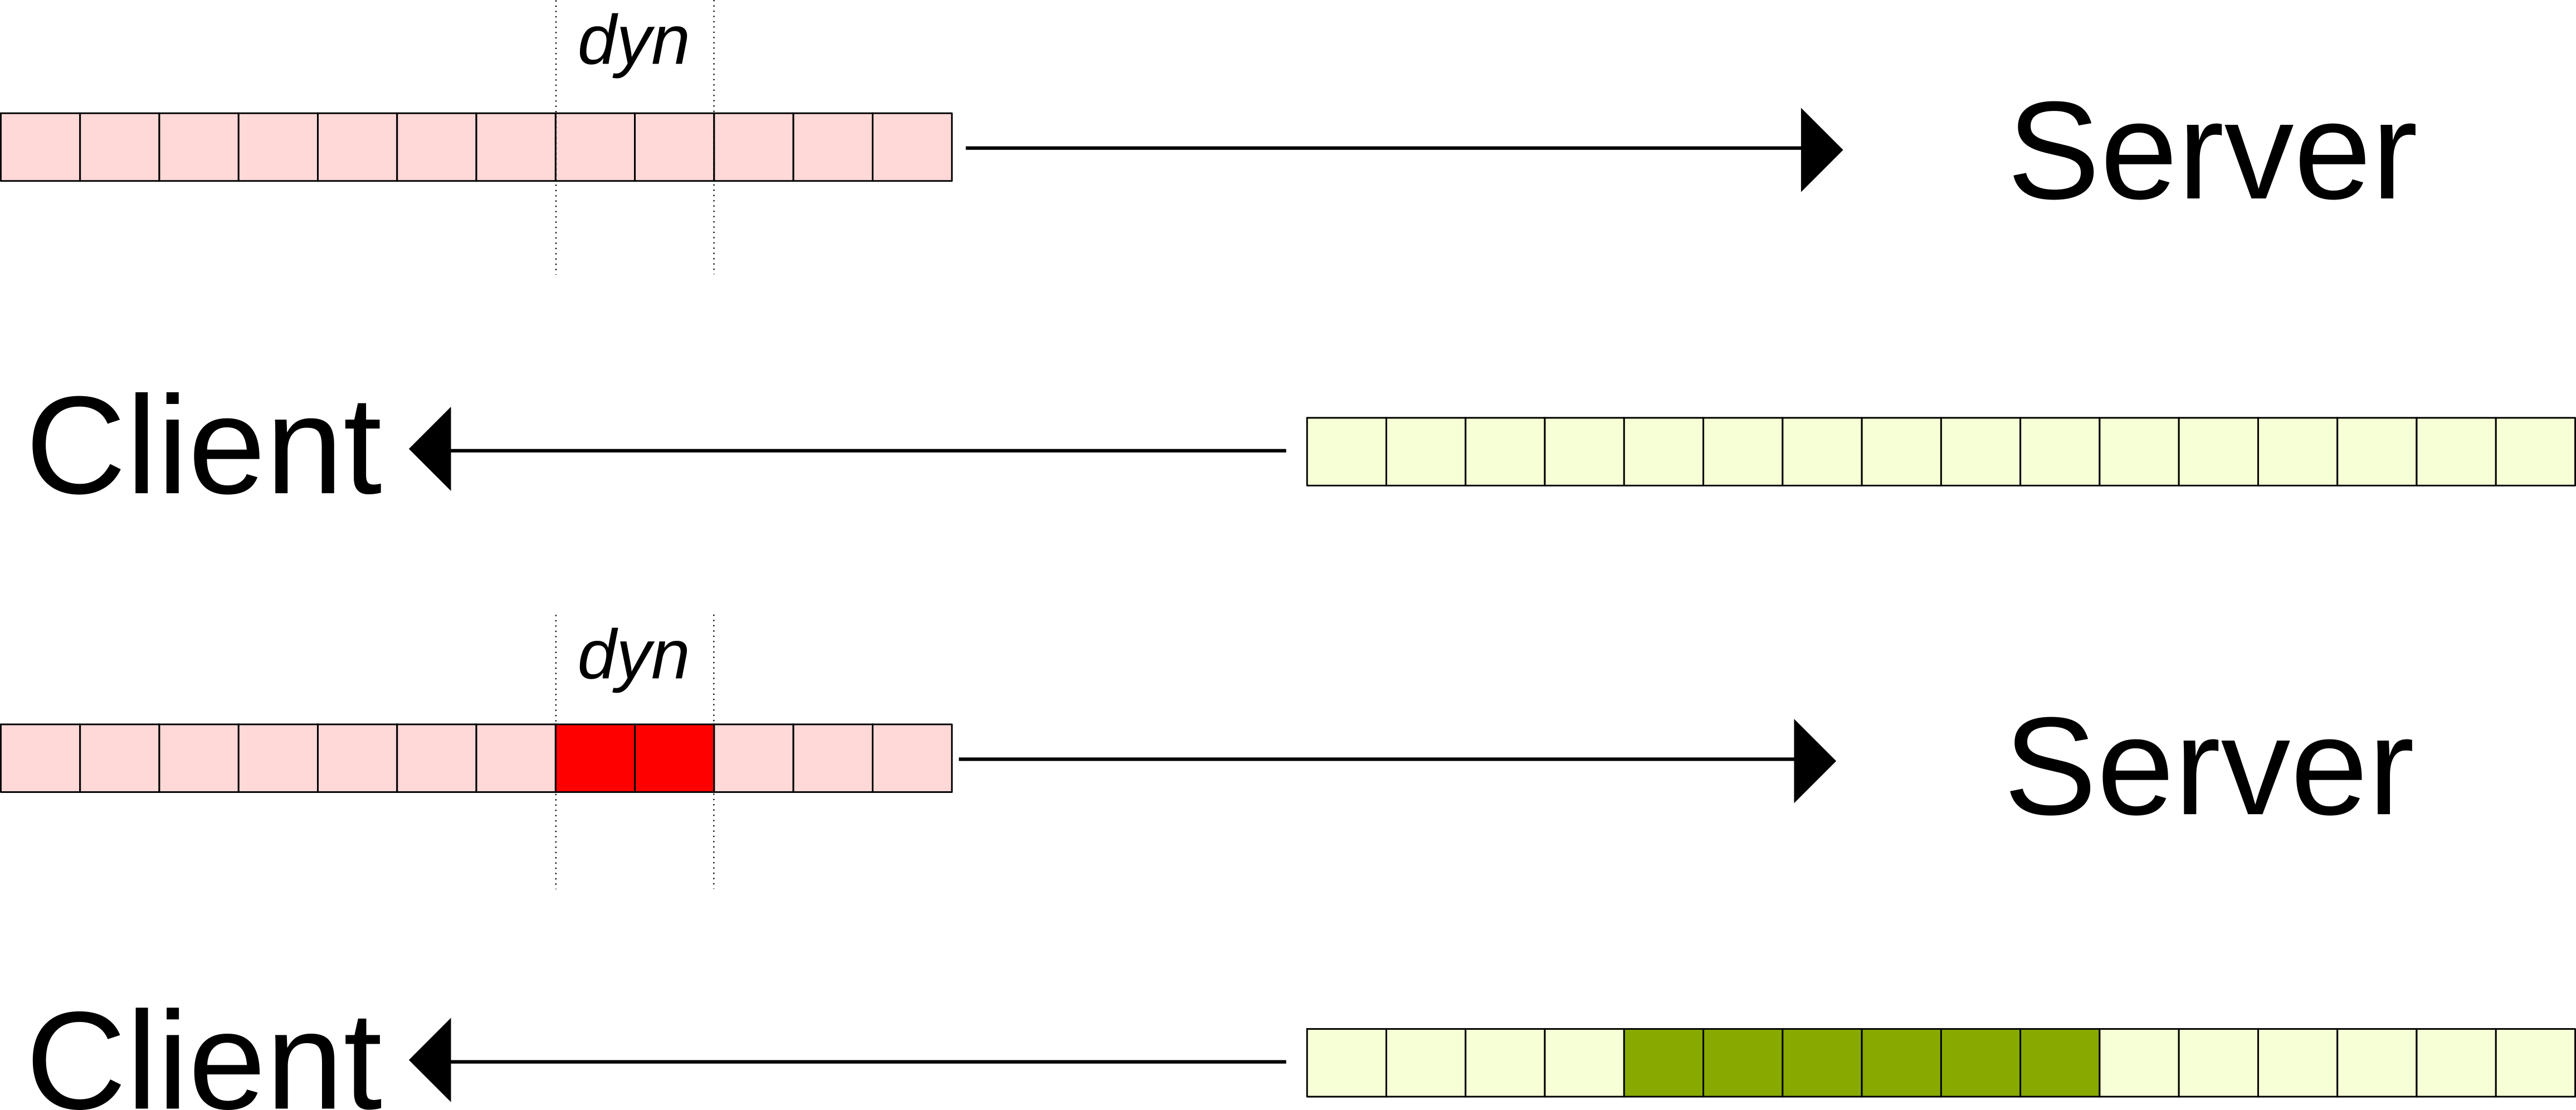
\includegraphics[scale=0.4]{modify.png}\end{center}

\end{frame}



\begin{frame}{Verifying Hypothesis}
\begin{center}
\scalebox{0.9}{
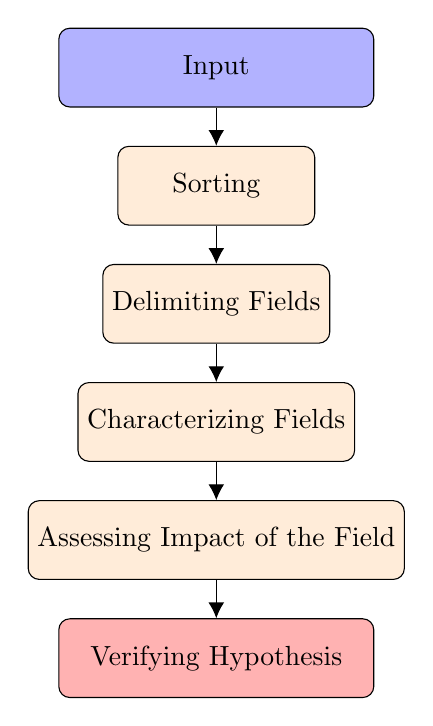
\begin{tikzpicture}[node distance=1.5cm,
    every node/.style={fill=white, font=\sffamily}, align=center]

\node (Input)             [activityStarts]              {Input};

\node (SI)     [process, below of=Input]          {Sorting};

\node (DF)     [process, below of=SI]          {Delimiting Fields};

\node (CF)     [process, below of=DF]          {Characterizing Fields};

\node (AI)     [process, below of=CF]          {Assessing Impact of the Field};

\node (VH)     [startstop, below of=AI]          {Verifying Hypothesis};

\draw[->]             (Input) -- (SI);
\draw[->]             (SI) -- (DF);
\draw[->]             (DF) -- (CF);
\draw[->]             (CF) -- (AI);
\draw[->]             (AI) -- (VH);
  \end{tikzpicture}}
  \end{center}
  
  \end{frame}
  
  \begin{frame}{Verifying Hypothesis}
  \begin{itemize}
  \item Change a static field

  $\Rightarrow$ get no error/timeout $\rightarrow$ False H
  
  \bigskip

  \item Put binary value in a text field
  
  $\Rightarrow$ get no error/timeout $\rightarrow$ False H
  \end{itemize}
  
  and a lot more !!!
  
  \end{frame}


\section{Future Work}
\begin{frame}

	\tableofcontents[currentsection]
\end{frame}

\begin{frame}{Future Work}
\begin{itemize}
\item Search Crucial Bytes 
\item 
\end{itemize}

\end{frame}

\begin{frame}{Conclusion}
\begin{itemize}
\item Good Points

\item Experience earned
\end{itemize}
\end{frame}

\end{document}
